%!TEX root = ../report.tex
\section{Methods} % (fold)
\label{sec:methods}
The LUDO player is consists of an artificial neural network that is evolved with a genetic algorithm (ANNGA Player).
	\subsection{Artificial Neural Network} % (fold)
	\label{sub:artificial_neural_network}
	A feedforward neural net with 9 inputs neurons, 3 hidden and 1 output is used \cite{kasper}. 
	Each input represents a situation of a brick of the player in the game. 
	The output is the goodness of a movement based on the input and the internal ANN weights (Fig. \ref{fig:ann_scheme}).
	\begin{figure}[ht]
		\centering
		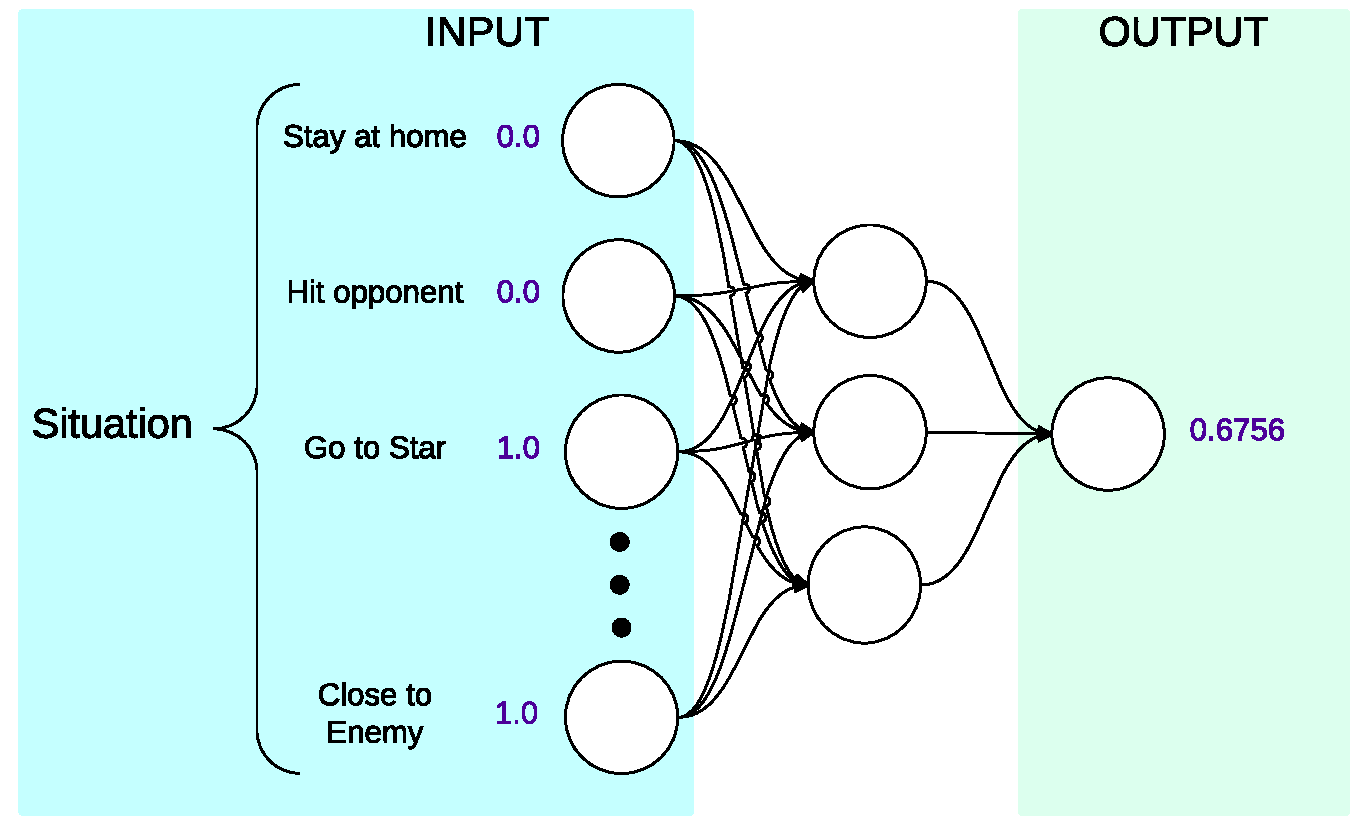
\includegraphics[width=\textwidth]{figures/ann_scheme}
		\caption{ANN representation for a possible situation and its output}
		\label{fig:ann_scheme}
	\end{figure}
	The net is trained with a sigmoid activation function (eq. \ref{eq:sigmoid_function}) so the output is a float number between 0 and 1.
	It is trained using backpropagation until a maximum defined error or a iteration limit is reached.
	\begin{equation}
		P(t)=\frac{1}{1+e^{-t}}
		\label{eq:sigmoid_function}
	\end{equation}

		\subsubsection{Inputs of the ANN} % (fold)
		\label{ssub:inputs}
		There are 9 input neurons, each neuron is connected uniquely to an occurrence inside the game. Each of the inputs is expressed in the table \ref{tab:ann_inputs}.
		\begin{table}[ht]
			\caption{Inputs of the ANN}
			\label{tab:ann_inputs}
			\centering
			\begin{tabular}{ c c }
			\textbf{Input} & \textbf{Description} \\
			\hline
				1 & Move the brick to goal \\
				2 & Hit opponent and send it to its home \\
				3 & Hit myself and go to home \\
				4 & Go to star \\
				5 & Go to globe \\
				6 & Go out home \\
				7 & Close to an enemy \\
				8 & Go to safe area \\
				9 & Move into the safe area \\
			\end{tabular}
		\end{table}
		% subsubsection inputs (end)

		\subsubsection{Backpropagation} % (fold)
		\label{ssub:backpropagation}
		During the game, the 9 inputs lead to 17 different situations. 
		A situation is defined as a combination of possible inputs. 
		For example, a situation in which a brick is \emph{close to an enemy} but also is \emph{in a star}. 
		However, there are also impossible situations as only \emph{Go out home} because when a brick is taken out of home, immediately hits a globe.
		
		When training the network, a desired output for an input is given.
		The training set is all the possible defined situations, in this case 17.
		And the desired output of each situation has to be chosen previously.
		As an example, the table \ref{tab:ann_training} shows possible situations and a possible desired outputs.
		\begin{table}[ht]
			\caption{Training example}
			\label{tab:ann_training}
			\centering
			\begin{tabular}{ c | c | c | c | c | c || c }
			\multicolumn{6}{ c || }{\textbf{Inputs}} & \textbf{Desired output} \\
			\hline
				 &\emph{Go to goal} & \emph{Hit opponent} & \emph{Close to Enemy} & ... & \emph{Go to star} & \\
				 \hline
				 & 1.0 & 0.0 & 0.0 & ... & 0.0 & 0.784 \\
				 & 0.0 & 1.0 & 0.0 & ... & 0.0 & 0.784 \\
				\textbf{Situations} & 0.0 & 0.0 & 1.0 & ... & 0.0 & 0.251 \\
				 & ... & ... & ... & ... & ... & ... \\
				 & 0.0 & 1.0 & 1.0 & ... & 1.0 & 0.969 \\
			\hline
			\end{tabular}
		\end{table}
		The ANN is trained with backpropagation until an maximum error of 0.001 is found or 5000 iterations are made.
		The pseudo code of the algorithm used for training a ANN when a new player is created is:
			\begin{enumerate}
				\item Create ANN with its structure (9,3,1).
				\item Define its ideal solution.
				\item Train the ANN with the ideal solution and the training set until the error is less than 0.001 or 5000 iterations are made.
			\end{enumerate}
		% subsubsection backpropagation (end)
		\subsubsection{Selecting which brick move} % (fold)
		\label{ssub:selecting_which_brick_move}
		The ANNGA player analyze the situation of each brick giving a numerical value of it. 
		The situations are compared and the highest score is the choice to move.
		If two situations have the same value, both situations are equally good and a random brick is moved.
		The pseudo code for the algorithm of choice is expressed as:
		\begin{enumerate}
			\item For each brick
			\begin{enumerate}
				\item Determine the situation
				\item Compute its value with the ANN
			\end{enumerate}
			\item Move the brick with the best situation
		\end{enumerate}
		% subsubsection selecting_which_brick_move (end)
	% subsection artificial_neural_network (end)

	\subsection{Genetic Algorithm} % (fold)
	\label{sub:genetic_algorithm}
	For training the ANN, an ideal solution for the 17 situation is given.
	The ideal situations are unknown and due to is a game of chance, there is not an optimal.
	However, different ideal solutions lead to unequal results.
	Depending on the type of the opponent, a better strategy is searched.
	For example, if the ANNGA player is playing against three pacifist players, a good strategy is not to take into account the possibility of being hit by the others. 
	The behavior of the ANNGA player is defined by the ideal solution for each situation and a GA is applied to find the most suitable strategy for each tournament.
		\subsubsection{Chromosome} % (fold)
		\label{ssub:chromosome}
		Each gene of the chromosome is the desired output for each situation defined in the ANN.
		This means that if 17 situations have been defined, the length of the chromosome is 17.
		Each gene means the importance adopted for a situation. 
		For example, a gene of 0.95 in \emph{Hit the opponent} means that the ANN gives a lot of importance to the possibility of hitting.
		A gene of 0.01 in \emph{Stay at home} and \emph{Go to globe} means that the choice of being at home is not the priority.
		% subsubsection chromosome (end)

		\subsubsection{Selection} % (fold)
		\label{ssub:selection}
		A population of 8 players with different chromosomes is initiated randomly \cite{koh}. 
		The size of the population is defined by the number of computer threads as will be explained in the implementation [\ref{sub:implementation}].
		Each player is made to play a defined number of games against other players and for each game some points are given.
		At the end of all the games, the two players with more points will become the mother and the father.
		Two ways of giving points have been experimented: (1) one point given if the game is won and (2) a proportional number of points depending on you position, being the first 3, second 2, third 1 while the looser doesn't receive any points.
		Despite the selection of the chromosome is the same the two strategies can lead to different results.
		% subsubsection selection (end)

		\subsubsection{Offspring} % (fold)
		\label{ssub:offspring}
		Once the mother and the father have been selected, the next generation can be made.
		The offspring is the population derived from the previous generation.
		An elitism of two-eighths is made.
		This means that, in the next generation, the father and the mother will remain the same.
		As there are 8 players, the other 6 are generated from them.
		As LUDO game is a game of chance, the players are made to play a defined number of games. This is known as a tournament.
		It has to be big enough to reduce the \emph{luck component} up to an acceptable limit.
		If the tournament have achieved this, doesn't make sense to keep other chromosomes different from the two best ones.
		Otherwise, this would mean give more \emph{opportunities} to a chromosome when it is supposed that the tournament should do that.
		Thus, only the father and the mother remain equal, the rest are changed.
		% subsubsection offspring (end)

		\subsubsection{Crossover} % (fold)
		\label{ssub:crossover}
		The chromosome of the other 6 players is created crossing the chromosomes of the parents.
		Two strategies have been implemented: (1) One point crossover and (2) uniform crossover.
		The uniform crossover have given better results and it is implemented making a random mask that chooses what genes from the father will be copied into the offspring. 
		The rest is copied from the mother.
		The number of genes copied from one of the parents respect to the total is known as the \emph{density} of the crossover.
		A density of 50\% has been applied meaning that for one children half of the genes are from the father and the other half from the mother.
		% subsubsection crossover (end)

		\subsubsection{Mutation} % (fold)
		\label{ssub:mutation}
		After the offspring is generated a mutation is made.
		For all the children, a mask that defines which gen will mutate is made. 
		The number of genes to mutate respect to the total is defined as \emph{density} of the mutation.
		A random density has been applied meaning that a random number of genes is mutated.
		For each gene to mutate, a random number is generated between two limits: \emph{max mutation} and \emph{min mutation}.
		In the experiments, due to the high speeds of the generations, a mutation between (-0.2, 0.2) is chosen.
		% subsubsection mutation (end)

		\subsubsection{Pseudo code for the GA} % (fold)
		\label{ssub:pseudo_code_for_the_ga}
		As the implementation of the game make use of all the threads in the computer, 8 ANNGA players play each own tournament against 3 SemiSmart players.
		So the pseudo code is:
		\begin{enumerate}
			\item Initialize 8 ANNGA players with random chromosomes.
			\item For each generation:
			\begin{enumerate}
				\item Each player, plays a defined number of games against 3 SemiSmarts.
				\item When finished, the number of points of each player is compared and the two best ones are selected.
				\item Create the offspring with the selected crossover method.
				\item Mutate the offspring.
				\item For the newborns, train their ANN with the new chromosome.
			\end{enumerate}

			\item When last generation is reached, the player with more points is put into the last tournament where the overall results are obtained.
		\end{enumerate}
		% subsubsection pseudo_code_for_the_ga (end)
	% subsection genetic_algorithm (end)
% section methods (end)